%%%--- Template for bachelor thesis at SfS, based on template
%%%--- for Diploma and Master thesis------
%%%------
\documentclass[11pt,a4paper,twoside,openright]{report}
\usepackage[english]{ETHDAsfs}%--> ETHDASA + fancyhdr + ... "umlaute"
%  + sfs-hyper -> hyperref 

\usepackage{pdfpages}%%to include the confirmation of originality (plagiarism
\usepackage{amsbsy}%% for \boldsymbol and \pmb{.}
\usepackage{amssymb}%% calls  amsfonts...
\usepackage{graphicx}%-- für PostScript-Grafiken (besser als  psfig!)
%\usepackage[draft]{graphicx} % grafics shown as boxes --> faster compilation
%
\usepackage[longnamesfirst]{natbib}%was {sfsbib}%- Für  Literatur-Referenzen
%           ^^^^^^^^^^^^^^ 1) "Hampel, Ronchetti, ..,"  2) "Hampel et al"
% Engineers (and other funny people) want to see [1], [2] 
% ---> use 'numbers' : \usepackage[longnamesfirst,number]{natbib}
%
%
\usepackage{texab}%- 'tex Abkürzungen' /u/sfs/tex/tex/latex/texab.sty
        %%- z.B.  \R, \Z, \Q, \Nat für reelle, ganze, rationale, natürl. Zahlen;
        %%-       \N   (Normalvert.)  \W == Wahrscheinlichkeit .....
        %%-  \med, \var, \Cov, \....
        %%-  \abs{x} == |x|   und   \norm{y} ==  || y ||   (aber anständig)
%% NOTE: texab contains many useful definitions and "shortcuts". It is
%% worth to open the file and have a look at them. HOWEVER, some
%% definitions are a bit can lead to conflicts with other packages. You
%% might for example want to comment out the line defininf \IF as an
%% operator when working with the algorithmic package, or to comment out
%% the line defining a command \Cite with working with the Biblatex package  
\usepackage{amsmath}
%\usepackage{mathrsfs}% Raph Smith's Formal Script font --> provides \mathscr
\usepackage[utf8]{inputenc}% <<------- Unicode, *NOT* iso-latin1 !
\usepackage{ae}% A[lmost] E[uropean] Fonts
\usepackage{enumerate}% Fuer selbstdefinierte Nummerierungen
%--------
\usepackage{relsize}%-> \smaller (etc) used here
\usepackage{color} %% to allow coloring in code listings
\usepackage{Sweave}
\usepackage{listings}% Fuer R-code, C-code, ....  and settings for these:

\usepackage{lineno}  %TODO comment this out when not needed anymore

\definecolor{Mygrey}{gray}{0.75}% for linenumbers only!
\definecolor{Cgrey}{gray}{0.4}% for comments
\lstloadlanguages{R}
%%--- first version of "listings of R"-style : ---------------------------
% %% using \smaller here: makes R code listings use a *small* font:
% \lstset{language=R,basicstyle=\smaller[2],commentstyle=\rmfamily\smaller,
%   showstringspaces=false,xleftmargin=4ex,
%   literate={<-}{{$\leftarrow$}}1 {~}{{$\sim$}}1}
% \lstset{escapeinside={(*}{*)}} % for (*\ref{ }*) inside lstlistings (Scode) 
%\newcommand{\lil}[1]{\lstinline|#1|}
%%--- newer version of "listings of R"-style : ---------------------------
\lstset{%% Help, e.g. --> https://en.wikibooks.org/wiki/LaTeX/Source_Code_Listings
language=R,
basicstyle=\ttfamily\scriptsize,%%- \small > \footnotesize > \scriptsize > \tiny
%commentstyle=\ttfamily\color{Cgrey},
commentstyle=\itshape\color{Cgrey},
numbers=left,
numberstyle=\ttfamily\color{Mygrey}\tiny,
stepnumber=1,
numbersep=5pt,
backgroundcolor=\color{white},
showspaces=false,
showstringspaces=false,
showtabs=false,
frame=single,
tabsize=2,
captionpos=b,
breaklines=true,
%breakatwhitespace=false,
keywordstyle={},
morekeywords={},
xleftmargin=4ex, 
literate={<-}{{$\leftarrow$}}1 {~}{{$\sim$}}1}
\lstset{escapeinside={(*}{*)}} % for (*\ref{ }*) inside lstlistings (Scode) 
%%----------------------------------------------------------------------------

%%------- Theoreme ---
\newtheorem{definition}{Definition}[subsection]
\newtheorem{lemma}[definition]{Lemma}
\newtheorem{theorem}[definition]{Theorem}
\newtheorem{Coro}[definition]{Corollary}
\theoremstyle{definition} 
\newtheorem{example}[definition]{Example}
\newtheorem*{note}{Note}
\newtheorem*{remark}{Remark}

\DeclareMathOperator*{\plim}{plim}
\def\MR#1{\href{http://www.ams.org/mathscinet-getitem?mr=#1}{MR#1}}

\newcommand{\Lecture}[3]{\marginpar{#3.#2.#1}}
\newcommand{\Fu}{\mathcal{F}}
\newcommand{\aatop}[2]{\genfrac{}{}{0pt}{}{#1}{#2}}

%\renewcommand{\theequation}{\arabic{equation}}
\numberwithin{equation}{subsection}
%\includeonly{}

%\pscompress %--compress the Epsf .ps files and produce .bb -- WHEN dvips is run
%\psdraft%--- for quick pre-viewing (only shows frames)

%%%%%%%%%%%%%%%%%%%%%%%%%%%%%%%%%%%%%%%%%%%%%%%%%
%%% Path for your figures                      %%%
%%%%%%%%%%%%%%%%%%%%%%%%%%%%%%%%%%%%%%%%%%%%%%%%%
% Set the paths where all figures are taken from:
% \graphicspath{{/u/mueller/MA/Figures1/}{/u/mueller/MA/Figures2/}}

%%%%%%%%%%%%%%%%%%%%%%%%%%%%%%%%%%%%%%%%%%%%%%%%%
%%% Define your own commands here             %%%
%%%%%%%%%%%%%%%%%%%%%%%%%%%%%%%%%%%%%%%%%%%%%%%%%
\newcommand{\Bruch}[2]{{}^{#1}\!\!/\!_{#2}}
\renewcommand{\labelenumi}{\roman{enumi}.)}





\begin{document}
\bibliographystyle{chicago}% ---> Hampel,F., E.Ronchetti,... W.Stahel(1986) ...
 %was \bibliographystyle{sfsbib}\citationstyle{dcu} %OR DEFAULT : \citationstyle{agsm}

\pagenumbering{roman}%- roman numbering for first few pages

%%%%%%%%%%%%%%%%%%%%%%%%%%%%%%%%%%%%%%%%%%%%%%%%%
%%% Title page                                %%%
%%%%%%%%%%%%%%%%%%%%%%%%%%%%%%%%%%%%%%%%%%%%%%%%%
 \period{Winter 2019} %e.g. Winter 2019
 \dasatype{Bachelor Thesis}
 \students{Nicolas Trutmann} %e.g. Patrick M\"uller
 \mainreaderprefix{Advisor:}
 \mainreader{placeholder} %e.g. Prof. Dr. Martin M\"achler
 \alternatereaderprefix{}
 \alternatereader{}
 \issuedate{placeholder} %e.g. September 15th 2019
 \submissiondate{placeholder} %e.g. February 31st 2019
 \title{Comparison of EM-algorithm and MLE using Cholesky decomposition} %title of your work

 \maketitle%- Titelseite wird abgeschlossen
 %%~~~~~~~~~~~~~~~~~~~~~~~~~~~~~~~~~~~~~~~~

%%%%%%%%%%%%%%%%%%%%%%%%%%%%%%%%%%%%%%%%%%%%%%%%%
%%% Insert here acknowledgements and abstract %%%
%%%%%%%%%%%%%%%%%%%%%%%%%%%%%%%%%%%%%%%%%%%%%%%%%
 \newpage
\begin{abstract}
	The intent of this work is to compare The EM algorithm to a MLE approach in the
	case of multivariate normal mixture models using the Cholesky decomposition.
	The EM algorithm is widely used in statistics and is proven to converge, 
	however in pathological cases convergence slows down considerably. 

	methods(not done)

	results(not done)
\end{abstract}

%%%%%%%%%%%%%%%%%%%%%%%%%%%%%%%%%%%%%%%%%%%%%%%%%
%%% Table of contents and list of figures and %%%   
%%% tables (no need to change this usually)   %%%
%%%%%%%%%%%%%%%%%%%%%%%%%%%%%%%%%%%%%%%%%%%%%%%%%
\newpage
\tableofcontents
\newpage
\listoffigures
\newpage
\listoftables
\cleardoublepage

\pagenumbering{arabic}%--- switch back to standard numbering 


%%%%%%%%%%%%%%%%%%%%%%%%%%%%%%%%%%%%%%%%%%%%%%%%%
%%% Your text... Either write here directly,  %%%
%%% or even better: write in separate files   %%%
%%% that you just have to include here.       %%% 
%%%%%%%%%%%%%%%%%%%%%%%%%%%%%%%%%%%%%%%%%%%%%%%%%
\linenumbers  %% TODO remove after not needed anymore
\chapter{Introduction to normal mixture models}% Umlaute work thanks to \inputencoding{..} % in main file

\section{Definitions}

here intro to normal mixtures

A good and thorough introductory book is the work of McLachlan and Peel 2000 and
the reader is encouraged to study that to learn in depth about normal mixtures. 
We will here give a short overwiev of normal mixtures to fix notation and nomenclature.

Let $ \mu \in \mathbb{R}^p , \quad \Sigma \in \mathbb{R}^{p \times p} $ and 
$ \phi(\mu, \Sigma) $ be the normal distribution with
mean $ \mu $ and covariance matrix $ \Sigma $.

Normal mixture model are designed for situations where we assume that a given 
dataset originates from more than one population of explaining variables.

$ \pmb{Y}_1, \dots , \pmb{Y}_n $

\begin{definition}
    Suppose we have a random sample $ \pmb{Y}_1, \dots , \pmb{Y}_n $ with 
    probability density function $ \pmb{Y}_j \sim f(y_j) $ on $\mathbb{R}^p$
    We assume that the density $ f(y_j) $ of $ \pmb{Y}_j $ can be written in
    the form 

    \[ f(y_j) = \sum_{i=1}^{K} \pi_i \phi_i (y_i) \]

    The $ \pi_i $ are called the component densities of the mixture.
\end{definition}

explain in scetch EM algo

EM has desirable qualities like proven convergence, (give reference to dempster 1977 paper)

explain idea to use parameter optimizer instead,
EM has pathological insufficiencies, like 'getting stuck' for many iterations.
we hope we need less iterations, and as concequence less time.
'special' idea: using cholesky decomp.


\section{choice of notation}

describe difference in notation between ceuleux \& govaert and our covariance matrix decomposition.

The classification of models in this paper relies heavily on the work of Celeux and Grovaert,
however, out of necessity for clarity, we break with their notation. 
So as to not confuse the reader we describe here in depth the differences in notation
between Celeux and Govaert and ours.

explanation for the volume, shape and orientation descriptors

The basis of classification in CnG is the decomposition of a symmetric matrix into
an orthogonal and a diagonal component.
A symmetric positive definite matrix $ \Sigma $ can be decomposed as follows
\[ \Sigma = \lambda \pmb{D} \pmb{A} \pmb{D}^{\top} \]
with $ \pmb{D} $ an orthogonal matrix and $ \pmb{A} $ a diagonal matrix and 
$ \lambda = \sqrt[\uproot{3}p]{det(\Sigma)} $ the $ p-th $ root of the determinant 
of $ \Sigma $.

This decomposition has an appealing geometric interpretation, with $ \pmb{D} $ 
as the \textit{orientation} of the distribution, $ \pmb{A} $ the \textit{shape}, and $ \lambda $
the \textit{volume}.
The problem of notation comes from standard conventions in linear algebra, where
the letters $A$ and $D$ are usually occupied by arbytrary and diagonal matrices 
respectively. Furthermore, we intend to apply a variant of the Cholesky decomposition
to $ \Sigma $, the $ \pmb{L}\pmb{D}\pmb{L}^{\top} $ decomposition.
This obviously raises some conflicts in notation.

Therefore we, from here on, when reffering to the decomposition as described
by cng, will use the following modification of notation:

\begin{align*} 
    \pmb{D} \longmapsto \pmb{Q} \\
    \pmb{A} \longmapsto \pmb{\Lambda} \\
    \lambda \longmapsto \alpha  \\
    \Sigma = \lambda \pmb{D} \pmb{A} \pmb{D}^{\top} =
        \alpha \pmb{Q} \pmb{\Lambda} \pmb{Q}^{\top}
\end{align*}

These were chosen according to general conventions of linear algebra.
$ \pmb{Q} $ is usually chosen for orthonormal matrices; $ \pmb{\Lambda} $ is 
often a choice for eigen vectors and $ \alpha $ was somewhat arbitrarily chosen.


make clear that the models can not be translated one to one to ldlt model

make nice table(maybe sideways to account for parameter list)


\begin{table}[!htb]
    \centering
\rotatebox{90}
{
    \begin{tabular}{| c | c c c c c c | c c c |}
        \hline
        Model & $\pmb{\Sigma}_k$ C\&G & volume & shape & orientation & parameters & count & $ \pmb{LDL}^\top $ & parameters & count \\
        \hline

        EII    & $ \alpha \pmb{I} $ & equal & equal & - & $ \alpha $ & 1 & same as C\&G & & \\
        VII    & $ \alpha_k \pmb{I} $         & variable & equal & - & $ \alpha_k $ & $ K $ & & & \\
        EEI    & $ \alpha \pmb{\Lambda} $     & equal & equal & coordinate axes & $ \alpha, \lambda_i $ & $ 1+p $ & & & \\
        VEI    & $ \alpha_k \pmb{\Lambda} $ & variable & equal & coordinate axes & $ \alpha_k, \lambda_{i}$ & $ K+p $ & & & \\
        EVI    & $ \alpha \pmb{\Lambda}_k $ &equal & variable & coordinate axes & $ \alpha, \lambda_{i,k} $ & $ 1+pK $ & & & \\
        VVI    & $ \alpha_k \pmb{\Lambda}_k $ & variable & variable & coordinate axes & $ \alpha_k, \lambda_{i,k} $ & $ K+pK $ & & & \\
        \hline
        EEE    & $ \alpha \pmb{Q \Lambda Q}^\top $ &equal & equal & equal & $ \alpha, \lambda_{i}, q_{i,j} $ & $ 1+p+p^2 $ & $ \alpha \pmb{LDL}^{\top} $ & & \\
        \hline
        EVE    & $ \alpha \pmb{Q \Lambda}_k \pmb{Q}^\top $ &equal & variable & equal & $ \alpha, \lambda_{i,k}, q_{i,j} $ & $ 1+pK+p^2 $ & doesn't exist & & \\
        \hline
        VEE    & $ \alpha_k \pmb{Q \Lambda Q}^\top $ & variable & equal & equal & $ \alpha_k, \lambda_{i}, q_{i,j} $ & $ K+p+p^2 $ & $ \alpha_k \pmb{LDL}^\top $ & & \\
        \hline
        VVE    & $ \alpha_k \pmb{Q \Lambda}_k \pmb{Q}^\top $ &variable & variable & equal & $ \alpha_k, \lambda_{i,k}, q_{i,j} $ & $ K+pK+p^2 $ & & & \\
        EEV    & $ \alpha \pmb{Q}_k \pmb{\Lambda} \pmb{Q}_k^\top $ &equal & equal & variable & $ \alpha, \lambda_{i}, q_{i,j,k} $ & $ 1+p+Kp^2 $ &    & & \\
        VEV    & $ \alpha_k \pmb{Q}_k \pmb{\Lambda} \pmb{Q}_k^\top $ &variable & equal & variable & $ \alpha_k, \lambda_{i}, q_{i,j,k} $ & $ K+p+Kp^2 $ & & & \\
        \hline
        EVV    & $ \alpha \pmb{Q}_k \pmb{\Lambda}_k \pmb{Q}_k^\top $ & equal & variable & variable & $ \alpha, \lambda_{i}, q_{i,j,k} $ & $ 1+pK+Kp^2 $ & $ \alpha \pmb{L}_k \pmb{D}_k \pmb{L}_k^\top $ & $ \lambda, d_{i,k}, l_{i,j,k}\ j>i $ & $ 1+pK+K\frac{p(p-1)}{2} $ \\
        VVV    & $ \alpha_k \pmb{Q}_k \pmb{\Lambda}_k \pmb{Q}_k^\top $ & variable & variable & variable & $ \alpha_k, \lambda_{i}, q_{i,j,k} $ & $ K+pK+Kp^2 $ & $ \alpha_k \pmb{L}_k \pmb{D}_k \pmb{L}_k^\top $ & $ \lambda_k, d_{i,k}, l_{i,j,k}\ j>i $ & $ K+pK+K\frac{p(p-1)}{2} $ \\
        \hline
    \end{tabular}

    \label{table:1}

}

\caption{Table of Parameters}

\end{table}


\clearpage

\section{problems of EM}


the EM algo has stalling problems especially close to a local optimum

show an example using nor1mix


\begin{Schunk}
\begin{Sinput}
> library("nor1mix")
> plot(MW.nm9, lty=2, col = "blue", p.norm=FALSE, p.comp=TRUE)
> set.seed(2019)
> x9 <- rnorMix(5000, MW.nm9)
> lines(density(x9), lwd=1.8)# "clearly" 3 components
\end{Sinput}
\end{Schunk}
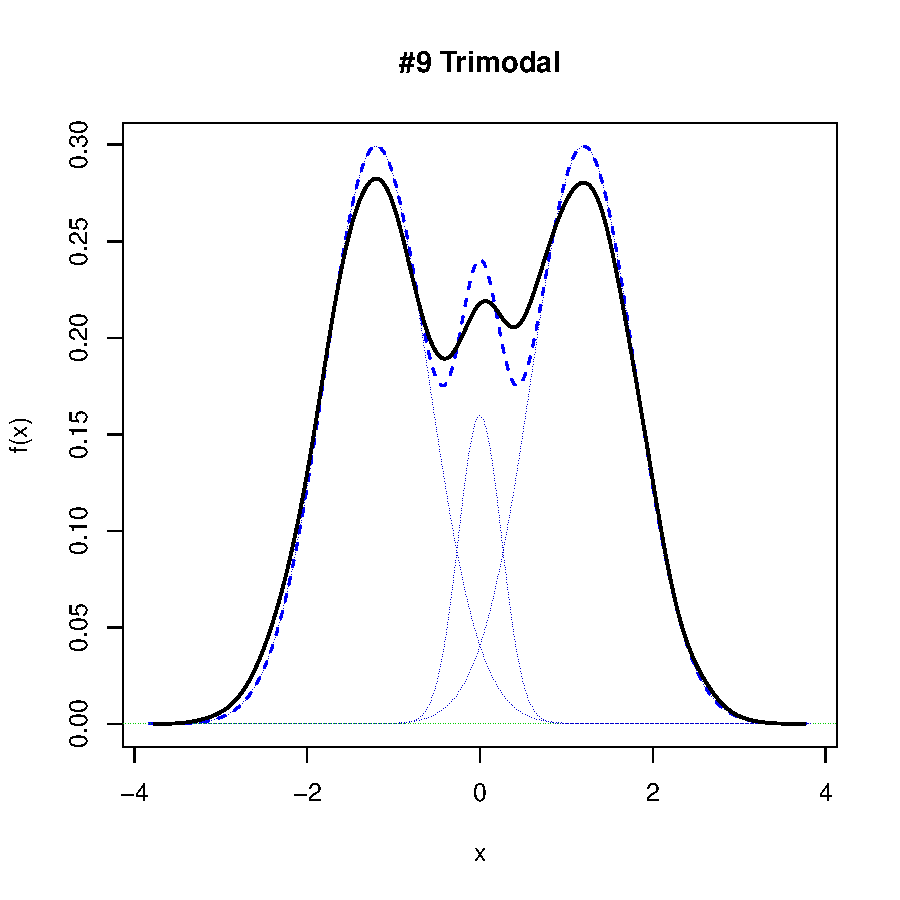
\includegraphics{chapter1-001}


then an illustration of MW examples of pathological cases


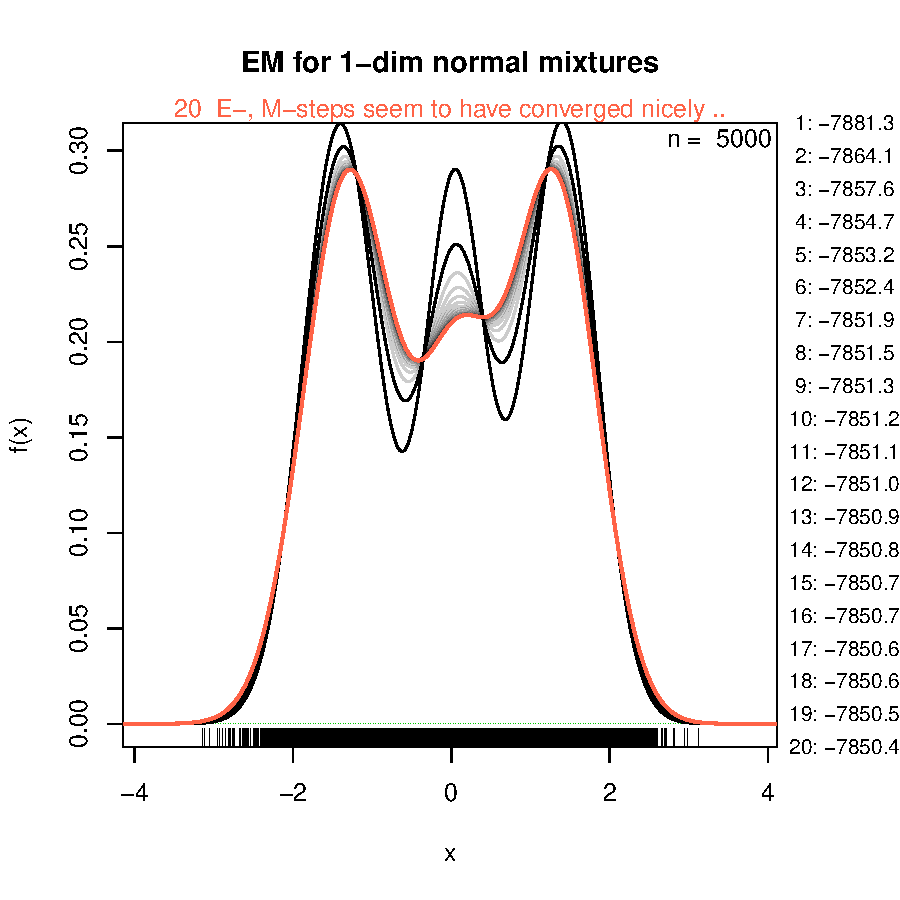
\includegraphics{chapter1-002}


yay, got figure to print. solution was use of fig=TRUE, instead of various mutations like figure=true.

here we see how change in loglik seems to stagnate. However, this does not stay that way, if we let EM run a bit further.

\begin{Schunk}
\begin{Sinput}
> r <- p.EMsteps(200, x9, nm1)
\end{Sinput}
\end{Schunk}
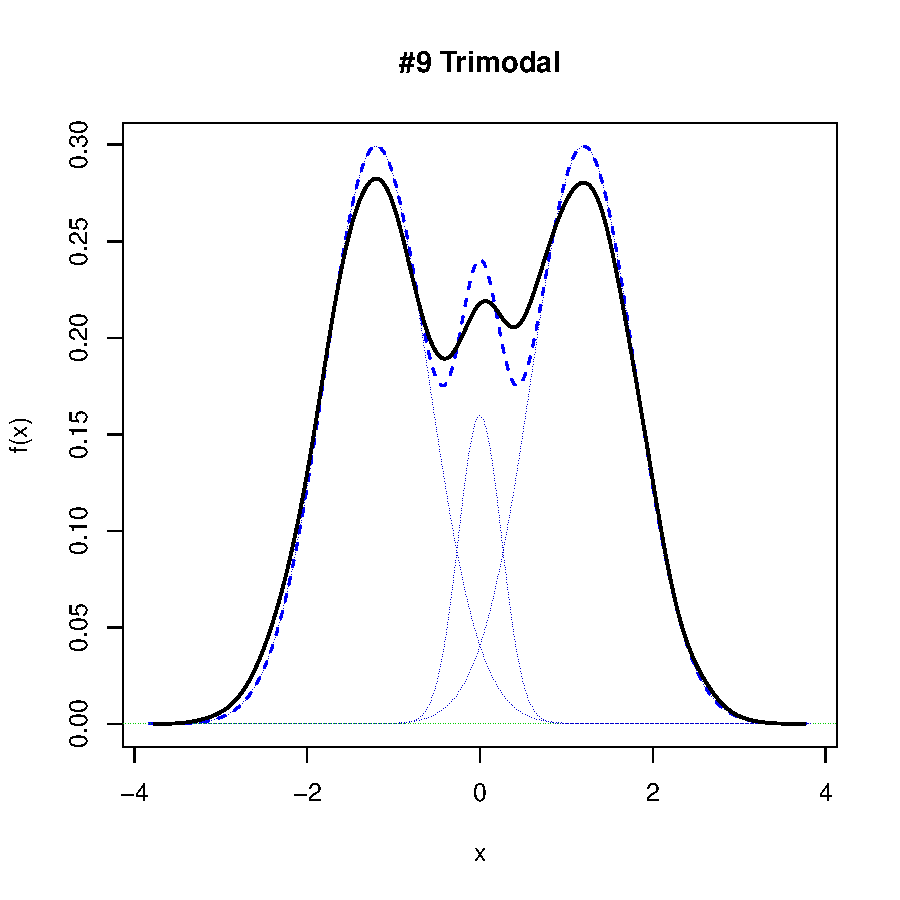
\includegraphics{chapter1-003}

to conclude example show part of mixest that shows it takes 1200 iterations to converge

In fact, it seems that the previous solution is a saddle point in the likelihood function, where EM has chronic problems continuing improvements.

should include animations?? like mix\_est\_1d.R line 249+24 lines

maybe show Marr Wand's examples of 'difficult' mixtures

give conclusion recapping the just demonstrated, and lead in for next chapter






\chapter{The {\tt norMmix} Package}

explain, that this package was written purposefully for this paper.

The norMmix package is constructed around the {\tt norMmix} object, that codifies a {\tt nor}mal {\tt M}ultivariate {\tt mix}ture model,  and the {\tt llnorMmix()} function.

quickly list contents of norMmix object

relies on {\tt optim()} generic optimizer. maximizes llnormix by varying model parameters.

since mclust is one of the more popular packages implementing the EM algo, we employ a lot of functions from mclust, to keep things around EM as similar as possible.

\section{concept of package} (this Section maybe one chapter earlier)

about Cholesky decomp as ldlt. has advantages: fast, parametrically parsimonious, can easily compute loglikelihood

maybe reread section in McLachlan about accelerating EM algo

not possible to sensibly compare normal mixtures except maybe a strange sorting algorithm using mahalanobis distance or Kullback-Leibler distance or similar(Hellinger), but not numerically sensible to integrate over potentially high-dimensional spaces.

So caomparison of algos done through throwing difficult mixtures and non-mixtures at it and hoping that norMmix finds better solutions than EM. So the criteria for "better fit" are 1. better log-likelihood 2. correct model, where EM fails.

\section{finer details of {\tt norMmix} package}




\chapter{Comparing Algotithms}

display abilities of norMmix on its own. can find correct models

maybe apply to MW[0-9] objects?

not sure


\chapter{Coclusions}

%% and more
% \include{....}
 
%%%%%%%%%%%%%%%%%%%%%%%%%%%%%%%%%%%%%%%%%%%%%%%%%
%%% Bibliography                              %%%
%%%%%%%%%%%%%%%%%%%%%%%%%%%%%%%%%%%%%%%%%%%%%%%%%
\addtocontents{toc}{\vspace{.5\baselineskip}}
% \cleardoublepage
\phantomsection
\addcontentsline{toc}{chapter}{\protect\numberline{}{Bibliography}}
\bibliography{References}
%% All books from our library (SfS) are already in a BiBTeX file
%% 'Assbib.bib' (included here as well), using
% \bibliography{myReferences,Assbib}
% ---------------------------------- instead of the above

%%%%%%%%%%%%%%%%%%%%%%%%%%%%%%%%%%%%%%%%%%%%%%%%% 
%%% Appendices (if needed, e.g. for R code)   %%%
%%%%%%%%%%%%%%%%%%%%%%%%%%%%%%%%%%%%%%%%%%%%%%%%%
\addtocontents{toc}{\vspace{.5\baselineskip}}
\appendix
\chapter{\Rp Code}
\section{{\tt llnorMmix}}

\begin{Schunk}
\begin{Soutput}
#### the llnorMmix function, calculating log likelihood for a given
#### parameter vector
## Author: Nicolas Trutmann 2019-07-06
## Log-likelihood of parameter vector given data
#
# par:   parameter vector
# tx:    transposed sample matrix
# k:     number of components
# model: assumed distribution model of normal mixture
# trafo: either centered log ratio or logit
llnorMmix <- function(par, tx, k,
                      trafo=c("clr1", "logit"),
                      model=c("EII","VII","EEI","VEI","EVI",
                              "VVI","EEE","VEE","EVV","VVV")
                      )
{
    stopifnot(is.matrix(tx),
              length(k <- as.integer(k)) == 1, k >= 1)
    p <- nrow(tx)
#    x <- t(x) ## then only needed in   (x-mu[,i])^2  i=1..k
    # 2. transform
    model <- match.arg(model)
    trafo <- match.arg(trafo)
    l2pi <- log(2*pi)
    # 3. calc log-lik
    # get w
    w <- if (k==1) 1
         else switch(trafo,
                     "clr1" = clr1inv (par[1:(k-1)]),
                     "logit"= logitinv(par[1:(k-1)]),
                     stop("invalid 'trafo': ", trafo)
         )
    # start of relevant parameters:
    f <- k + p*k # weights -1 + means +1 => start of alpha
    # get mu
    mu <- matrix(par[k:(f-1L)], p,k)
    f1 <- f      # end of alpha if uniform
    f2 <- f+k-1L # end of alpha if var
    f1.1 <- f1 +1L # start of D. if alpha unif.
    f2.1 <- f1 + k # start of D. if alpha variable
    f11 <- f1 + p-1    # end of D. if D. uniform and alpha uniform
    f12 <- f1 +(p-1)*k # end    D. if D.   var   and alpha unif.
    f21 <- f2 + p-1    # end of D. if D. uniform and alpha variable
    f22 <- f2 +(p-1)*k # end of D. if D.   var   and alpha var.
    f11.1 <- f11 +1L # start of L if alpha unif  D unif
    f21.1 <- f21 +1L # start of L if alpha var   D unif
    f12.1 <- f12 +1L # start of L if alpha unif  D var
    f22.1 <- f22 +1L # start of L if alpha var   D var
    f111 <- f11 +   p*(p-1)/2 # end of L if alpha unif  D unif
    f211 <- f21 +   p*(p-1)/2 # end of L if alpha var   D unif
    f121 <- f12 + k*p*(p-1)/2 # end of L if alpha unif  D var
    f221 <- f22 + k*p*(p-1)/2 # end of L if alpha var   D var
    # initialize f(tx_i) i=1..n  vector of density values
    invl <- 0
    # calculate log-lik, see first case for explanation
    switch(model,
    "EII" = {
        alpha <- par[f]
        invalpha <- exp(-alpha)# = 1/exp(alpha)
        for (i in 1:k) {
            rss <- colSums(invalpha*(tx-mu[,i])^2)
            # this is vector of length n=sample size
            # calculates (tx-mu)t * Sigma^-1 * (tx-mu) for diagonal
            # cases.
            invl <- invl+w[i]*exp(-0.5*(p*(alpha+l2pi)+rss))
            # adds likelihood of one component to invl
            # the formula in exp() is the log of likelihood
            # still of length n
        }
    },
    # hereafter differences are difference in dimension in alpha and D.
    # alpha / alpha[i] and D. / D.[,i]
    "VII" = {
        alpha <- par[f:f2]
        for (i in 1:k) {
            rss <- colSums((tx-mu[,i])^2/exp(alpha[i]))
            invl <- invl+w[i]*exp(-0.5*(p*(alpha[i]+l2pi)+rss))
        }
    },
    "EEI" = {
        alpha <- par[f]
        D. <- par[f1.1:f11]
        D. <- c(-sum(D.),D.)
        D. <- D.-sum(D.)/p
        invD <- exp(alpha+D.)
        for (i in 1:k) {
            rss <- colSums((tx-mu[,i])^2/invD)
            invl <- invl+w[i]*exp(-0.5*(p*(alpha+l2pi)+rss))
        }
    },
    "VEI" = {
        alpha <- par[f:f2]
        D. <- par[f2.1:f21]
        D. <- c(-sum(D.), D.)
        D. <- D.-sum(D.)/p
        for (i in 1:k) {
            rss <- colSums((tx-mu[,i])^2/exp(alpha[i]+D.))
            invl <- invl+w[i]*exp(-0.5*(p*(alpha[i]+l2pi)+rss))
        }
    },
    "EVI" = {
        alpha <- par[f]
        D. <- matrix(par[f1.1:f12],p-1,k)
        D. <- apply(D.,2, function(j) c(-sum(j), j))
        D. <- apply(D.,2, function(j) j-sum(j)/p)
        for (i in 1:k) {
            rss <- colSums((tx-mu[,i])^2/exp(alpha+D.[,i]))
            invl <- invl+w[i]*exp(-0.5*(p*(alpha+l2pi)+rss))
        }
    },
    "VVI" = {
        alpha <- par[f:f2]
        D. <- matrix(par[f2.1:f22],p-1,k)
        D. <- apply(D.,2, function(j) c(-sum(j), j))
        D. <- apply(D.,2, function(j) j-sum(j)/p)
        for (i in 1:k) {
            rss <- colSums((tx-mu[,i])^2/exp(alpha[i]+D.[,i]))
            invl <- invl+w[i]*exp(-0.5*(p*(alpha[i]+l2pi)+rss))
        }
    },
    # here start the non-diagonal cases. main difference is the use
    # of backsolve() to calculate tx^t Sigma^-1 tx, works as follows:
    # assume Sigma = L D L^t, then Sigma^-1 = (L^t)^-1 D^-1 L^-1
    # y = L^-1 tx  => tx^t Sigma^-1 tx = y^t D^-1 y
    # y = backsolve(L., tx)
    "EEE" = {
        alpha <- par[f]
        D. <- par[f1.1:f11]
        D. <- c(-sum(D.), D.)
        D. <- D.-sum(D./p)
        invD <- exp(alpha+D.)
        L. <- diag(1,p)
        L.[lower.tri(L., diag=FALSE)] <- par[f11.1:f111]
        for (i in 1:k) {
            rss <- colSums(backsolve(L.,(tx-mu[,i]), upper.tri=FALSE)^2/invD)
            invl <- invl+w[i]*exp(-0.5*(p*(alpha+l2pi)+rss))
        }
    },
    "VEE" = {
        alpha <- par[f:f2]
        D. <- par[f2.1:f21]
        D. <- c(-sum(D.), D.)
        D. <- D.-sum(D./p)
        L. <- diag(1,p)
        L.[lower.tri(L., diag=FALSE)] <- par[f21.1:f211]
        for (i in 1:k) {
            rss <- colSums(backsolve(L., (tx-mu[,i]), upper.tri=FALSE)^2/exp(alpha[i]+D.))
            invl <- invl+w[i]*exp(-0.5*(p*(alpha[i]+l2pi)+rss))
        }
    },
    "EVV" = {
        alpha <- par[f]
        D. <- matrix(par[f1.1:f12],p-1,k)
        D. <- apply(D.,2, function(j) c(-sum(j), j))
        D. <- apply(D.,2, function(j) j-sum(j)/p)
        L.temp <- matrix(par[f12.1:f121],p*(p-1)/2,k)
        for (i in 1:k) {
            L. <- diag(1,p)
            L.[lower.tri(L., diag=FALSE)] <- L.temp[,i]
            rss <- colSums(backsolve(L., (tx-mu[,i]), upper.tri=FALSE)^2/exp(alpha+D.[,i]))
            invl <- invl+w[i]*exp(-0.5*(p*(alpha+l2pi)+rss))
        }
    },
    "VVV" = {
        alpha <- par[f:f2]
        D. <- matrix(par[f2.1:f22],p-1,k)
        D. <- apply(D.,2, function(j) c(-sum(j), j))
        D. <- apply(D.,2, function(j) j-sum(j)/p)
        invalpha <- exp(rep(alpha, each=p)+D.)
        L.temp <- matrix(par[f22.1:f221],p*(p-1)/2,k)
        L. <- diag(1,p)
        for (i in 1:k) {
            L.[lower.tri(L., diag=FALSE)] <- L.temp[,i]
            rss <- colSums(backsolve(L., (tx-mu[,i]), upper.tri=FALSE)^2/invalpha[,i])
            invl <- invl+w[i]*exp(-0.5*(p*(alpha[i]+l2pi)+rss))
        }
    },
    ## otherwise
    stop("invalid model:", model)
    )
    ## return  sum_{i=1}^n log( f(tx_i) ) :
    sum(log(invl))
}
sllnorMmix <- function(x, obj, trafo=c("clr1", "logit")) {
    stopifnot(is.character(model <- obj$model))
    trafo <- match.arg(trafo)
    llnorMmix(nMm2par(obj, model=model),
              tx = t(x), k = obj$k, model=model, trafo=trafo)
}
## log-likelihood function relying on mvtnorm function
#
# par:   parameter vector as calculated by nMm2par
# x:     matrix of samples
# k:     number of cluster
# trafo: transformation of weights
# model: assumed model of the distribution
llmvtnorm <- function(par, x, k,
                      trafo=c("clr1", "logit"),
                      model=c("EII","VII","EEI","VEI","EVI",
                              "VVI","EEE","VEE","EVV","VVV")
              )
{
    stopifnot(is.matrix(x),
              length(k <- as.integer(k)) == 1, k >= 1)
    model <- match.arg(model)
    trafo <- match.arg(trafo)
    p <- ncol(x)
    nmm <- par2nMm(par, p, k, model=model, trafo=trafo)
    ## FIXME (speed!):  dmvnorm(*, sigma= S) will do a chol(S) for each component
    ## -----  *instead* we already have LDL' and  chol(S) = sqrt(D) L' !!
    ## another par2*() function should give L and D, or from that chol(Sagma), rather than Sigma !
    w <- nmm$w
    mu <- nmm$mu
    sig <- nmm$Sigma
    y <- 0
    for (i in 1:k) {
        y <- y + w[i]*mvtnorm::dmvnorm(x,mean=mu[,i],sigma=sig[,,i])
    }
    sum(log(y))
}
\end{Soutput}
\end{Schunk}

\section{Example Simulation Script}

% TODO:
here e.g. 2init.R and write some remarks on it.

% outcommented \chapter{Complementary information}
\label{app:complement}

Additional material. For example long mathematical derivations could be
given in the appendix. Or you could include part of your code that is
needed in printed form. You can add several Appendices to your thesis (as
you can include several chapters in the main part of your work).

\section{Including \Rp code with verbatim}
A simple (rather too simple, see~\ref{App:listings}) way to include code or
{\it R} output is to use 
\texttt{verbatim}. It just prints the text however it is (including all
spaces, ``strange'' symbols,...) in a slightly different font.
\begin{verbatim}
## loading packages
library(RBGL)
library(Rgraphviz)
library(boot)

## global variables
X_MAX <- 150

   This allows me to put as many s  p a   c es   as I want.
I can also use \ and ` and & and all the rest that is usually only 
accepted in the math mode.

I can also make as 
                  many 
             line 
    breaks as 
I want... and
             where I want. 
\end{verbatim}

But really recommended,  much better is the following:

\section{Including \Rp code with the \emph{listings} package}\label{App:listings}
However, it is much nicer to use the \emph{listings} package to include \Rp
code in your report. It allows you to number the lines, color the comments
differently than the code, and so on.
All the following is produced by simply writing

or \verb!\lstinputlisting{/u/maechler/R/Pkgs/sfsmisc/R/ellipse.R}! :

\lstinputlisting{ellipse.R}% was /u/maechler/R/Pkgs/sfsmisc/R/ellipse.R

\section{Using Sweave to include \Rp code (and more) in your report}
The easiest (and most elegant) way to include \Rp code and its output (and
have all your figures up to date with your report) is to use Sweave. You
can find an introduction Sweave in \texttt{/u/sfs/StatSoftDoc/Sweave/Sweave-tutorial.pdf}.

%%% Local Variables: 
%%% mode: latex
%%% TeX-master: "BachelorThesisSfS"
%%% End: 

% outcommented \chapter{2nd Appendix: More sophisticated R code listing} \label{appendix-more-R}

Chapter-wise listing of parts of R code, using
\begin{itemize}
\item \texttt{firstline=n1}
\item \texttt{lastline=n2}
\item \texttt{title=<text>}
\end{itemize}
e.g., for the first example below
\begin{verbatim}
\lstinputlisting[firstline=1,lastline=32,
                 title= \texttt{read\_irwls\_fn.R}]{../RCode/read_irwls_fn.R}
\end{verbatim}

% \section{Chapter 2} \label{app 2}

% \lstinputlisting[firstline=1,lastline=77,
% title=\texttt{analytic\_efficiency.R}]{../RCode/analytic_efficiency.R}
% %\lstinputlisting[firstline=,lastline=]{../RCode/???.R}

\bigskip% or even  \clearpage

%-----------------------------------------------------------------------------------------
\section{Chapter 5} \label{app 5}

% \lstinputlisting[firstline=1,lastline=71,
%                  title=\texttt{loss-fn\_rotated.R}]{../RCode/loss-fn_rotated.R}
%\lstinputlisting[firstline=1,lastline=32,
%                 title= \texttt{read\_irwls\_fn.R}]{../RCode/read_irwls_fn.R}

\medskip
                 
%\lstinputlisting[firstline=1,lastline=45,title=\texttt{plot.psi.R}]{../RCode/plot.psi.R}
%\lstinputlisting[firstline=,lastline=]{../RCode/???.R}
%\lstinputlisting[firstline=,lastline=]{../RCode/???.R}

% \clearpage
%-----------------------------------------------------------------------------------------
% \section{Chapter 7} \label{app 7}

% \lstinputlisting[firstline=1,lastline=35,
%                  title= \texttt{stat.test} from \texttt{lmrob2-fn.R}]{../RCode/lmrob2-fn.R}
% \lstinputlisting[firstline=41,lastline=194,
%                  title=\texttt{M.optimal.ms} from \texttt{lmrob2-fn.R}]{../RCode/lmrob2-fn.R}
%\lstinputlisting[firstline=,lastline=]{../RCode/???.R}
%-----------------------------------------------------------------------------------------

%%% Local Variables:
%%% mode: latex
%%% TeX-master: "MasterThesisSfS"
%%% End:


%%%%%%%%%%%%%%%%%%%%%%%%%%%%%%%%%%%%%%%%%%%%%%%%%% 
%%% Declaration of originality (Do not remove!)%%%
%%%%%%%%%%%%%%%%%%%%%%%%%%%%%%%%%%%%%%%%%%%%%%%%%%
%% Instructions:
%% -------------
%% fill in the empty document confirmation-originality.pdf electronically
%% print it out and sign it
%% scan it in again and save the scan in this directory with name
%% confirmation-originality-scan.pdf 
%%
%% General info on plagiarism:
%% https://www.ethz.ch/students/en/studies/performance-assessments/plagiarism.html 
\cleardoublepage
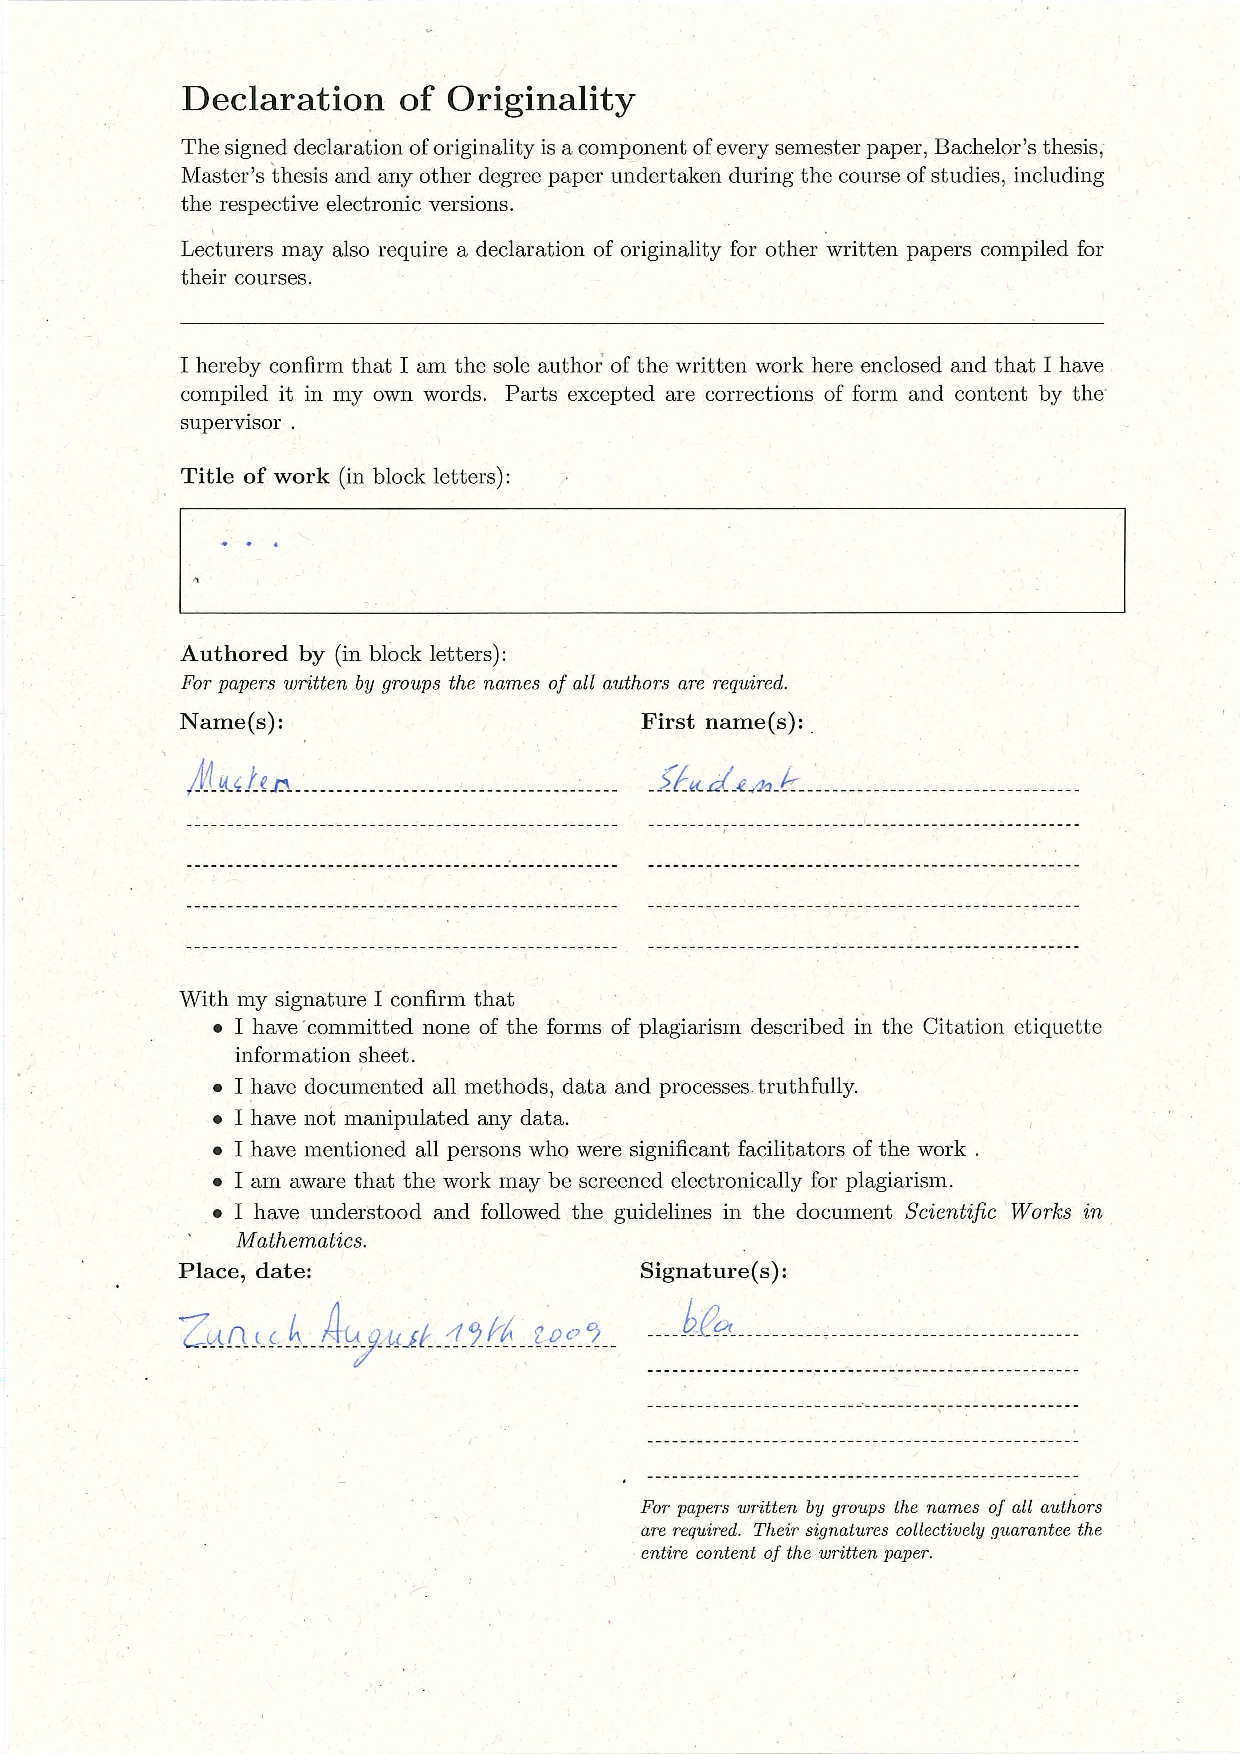
\includepdf[pages={-}, frame=true,scale=1]{confirmation-originality-scan.pdf}
\end{document}
